\chapter{Технологический раздел}

\section{Реализация алгоритма шифрования}

В листингах \ref{lst:l1}~--~\ref{lst:l2} приведена реализация алгоритма шифрования машины <<Энигма>>.
\begin{lstlisting}[language=C, label=lst:l1, caption={Реализация алгоритма шифрования (начало)}]
void shift_by_one(int* rotor, size_t size) {
    int last = rotor[size - 1];

    for (size_t i = size - 1; i >= 1; i--) {
        rotor[i] = rotor[i - 1];
    }

    rotor[0] = last;
}

size_t get_index(const int* rotor, size_t size, int val) {
    for (size_t i = 0; i < size; i++) {
        if (rotor[i] == val) {
            return i;
        }
    }

    return -1;
}

unsigned char* encode_enigma(enigma_t* enigma, unsigned char* msg, size_t size) {
    unsigned char* res = calloc(size, sizeof(unsigned char));

    enigma->counter = 1;
    for (size_t i = 0; i < size; i++, enigma->counter++) {
        int code = msg[i];

        code = enigma->panel[code];
\end{lstlisting}

\newpage
        
\begin{lstlisting}[language=C, label=lst:l2, caption={Реализация алгоритма шифрования (продолжение \ref{lst:l1})}]

		for (size_t j = 0; j < enigma->size_rotors; j++) {
            code = enigma->rotors[j][code];
        }

        code = enigma->reflector[code];

        for (int j = enigma->size_rotors - 1; j >= 0; j--) {
            code = get_index(enigma->rotors[j], enigma->size_alphabet, code);
        }

        code = enigma->panel[code];

        res[i] = code;

        shift_by_one(enigma->rotors[0], enigma->size_alphabet);
        for (size_t j = 1; j < enigma->size_rotors; j++) {
            if (enigma->counter % (enigma->size_alphabet * j) == 0) {
                shift_by_one(enigma->rotors[j], enigma->size_alphabet);
            }
        }
    }

    return res;
}
\end{lstlisting}

\section{Тестирование}
Корректность алгоритма проверялось путем применения дешифрации на шифрованное сообщение.

Тестирование было проведено на файлах с типами:

\begin{enumerate}[label=\arabic*)]
	\item текстовый (txt);
	\item графический (jpg, png);
	\item архив (zip);
	\item исходного кода (c);
	\item несуществующий (cumberbatch).
\end{enumerate}

В таблице \ref{tbl:test} представлены тестовые данные.

\begin{table}[H]
	\begin{center}
		\centering
		\caption{Тестовые данные}
		\label{tbl:test}
		\begin{tabular}{|c|c|c|} 
			
			\hline
			\multicolumn{1}{|c|}{Номер теста}
			&  \multicolumn{1}{c|}{Тип файла} &  \multicolumn{1}{c|}{Содержимое файла}\\
			\hline
			
			1& txt &  {\specialcell{зачем это все, если можно\\просто лечь на спину....7....}} \\ \hline
			
			2& txt &  {\specialcell{why do all this if you can\\just lie on your back....7....}} \\ \hline
			
			3& txt &  $\varnothing$\\ \hline
			
			4& zip & Файлы с тестов 1 и 5 \\ \hline
			
			5& jpg & {\specialcell{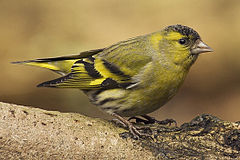
\includegraphics[width=1in]{inc/img/test.jpg}}} \\ \hline
			
			6& c & Файл исходного кода текущей л/р \\ \hline
			
			7& cumberbatch & {\specialcell{On Пон, 27 Мар 2023 10:48:02 +0300\\
 Толпинская Наталья Борисовна wrote:\\
Добрый день!Задание на Лаб 7\\
On Пон, 13 Мар 2023 10:02:34 +0300\\
Толпинская Наталья Борисовна wrote:\\
Добрый день!Задание на первую часть 6 лаб раб.\\
выполнять надо на занятии! Н.Б. Толпинская}} \\ \hline
			
			8& png & {\specialcell{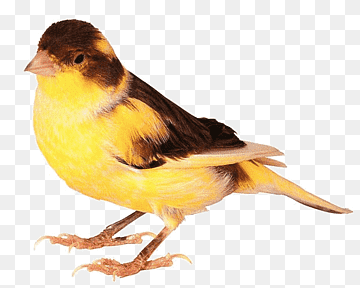
\includegraphics[width=1in]{inc/img/test_05.png}}} \\ \hline
			
		\end{tabular}
	\end{center}
\end{table}
